\chapter{Tracing with ftrace}
% Capitolo Marco Perronet
\label{chap:ftrace}
Kernel debugging is a big challenge even for the most experienced kernel developers. The problem is that if the system has, for example, latencies or synchronization issues (undetected race conditions), it's really hard to pinpoint where they're coming from. Which subsystems are involved? In which conditions does the problem arise? When the system is running, not always there is a way to know the answer. Ftrace is a debugger designed specifically to solve the issue and make the developer's life easier. It's also a great educational tool, not just to peek at what happens in the kernel, but also to help approach the source code by observing the function flow.

The name comes from ``function tracer'', which is one of its features, but it has many others. Each mode of tracing is simply called a \textit{tracer}, and each one comes with many options to tweak it. They can do function tracing, event tracing, measure context switch time or the time in which interrupts are disabled. Ftrace is also very extensible because it's possible to write new tracers that can be added like a module.

As anticipated, one of the objectives of the thesis is to document events related with scheduling. To understand what they do and why they are useful, it's necessary to understand ftrace, which is the tool that uses them.
\section{How does it work?}
\label{sec:how_does_it_work}

Tracing means recording events that occur at runtime in order to analyze the code's behavior and performance. More generally, this is called \textit{software profiling} ans it's implemented with different techniques. In our case, it's achieved by the means of \textit{code instrumentation}, which consists in adding instructions to the source code or its binary in order to profile it. There are two main ways of using ftrace, and they use two different instrumentation techniques:
\begin{itemize}
    \item Function tracing, using \verb|gcc|'s code instrumentation mechanism activated by compiling with the \verb|-pg| option.
    \item Event tracing, using \textit{tracepoints} in the source code.
\end{itemize}
Function tracing uses a form of dynamic profiling: this means that the tracing instructions can be toggled at runtime in the binary executable, without the need to recompile the code. The way this works is that, while compiling, \verb|gcc| adds extra \verb|NOP| assembly instructions at the beginning of every function. The position of these instructions is then saved in the binary itself, so that it will be possible to change these \verb|NOP|s into something else. This is exactly what ftrace does: it toggles tracing by changing these instructions at runtime; they are converted to \verb|JMP| instructions to tracing functions, and then back to \verb|NOP| to disable tracing. For this reason, this instrumentation technique is called \textit{runtime injection}. This approach has two main advantages: 
\begin{itemize}
    \item Since we can toggle tracing at runtime, there is zero overhead when it's disabled (so 99\% of the time).
    \item It's possible to filter what is being traced: we could dynamically activate tracing only on functions from a single subsystem, or on one function alone.
\end{itemize}

Event tracing, on the other hand, is a little different and it's less efficient than function tracing because it doesn't use runtime injection. Instead, it uses tracepoints directly in the c code, which makes it static. Tracepoints are simply direct calls to tracing function, which will gather some information through parameters and then write it in the trace output, along with the event name. Since this mechanism is static, the whole kernel must be recompiled to toggle the tracepoints: this is done by simply toggling the \verb|CONFIG_TRACEPOINTS| macro in the configuration before compiling. Let's take two scheduling events as an example: \verb|sched_stat_runtime| and \verb|sched_migrate_task|. The first happens in a specific point of the scheduler code and contains core scheduling information about a given process; the second happens upon migration of a task and contains information such as the CPU the thread was migrated to. They are called in the code like this:
\begin{code}
// curtask and curr are task_structs, delta_exec is the difference in runtime since the last timer interrupt. 
trace_sched_stat_runtime(curtask, delta_exec, curr->vruntime);
// p is a task_struct, new_cpu is the CPU the thread migrated to
trace_sched_migrate_task(p, new_cpu);
\end{code}
When these events happen, they will appear in the trace output like this:
\begin{Verbatim}[xleftmargin=-2cm,fontsize=\footnotesize]
# The format is name, pid, cpu, timestamp, event name, event information 
AudioIPC-1849  [002] 21448.743195: sched_stat_runtime:   comm=AudioIPC Callba pid=1849 runtime=104248 [ns] vruntime=3462508278368 [ns]
AudioIPC-1849  [002] 21448.743174: sched_migrate_task:   comm=AudioIPC Client pid=26778 prio=120 orig_cpu=3 dest_cpu=0
\end{Verbatim} 

Notice how all the information can be found through the parameters: command, pid, runtime and priority can all be found directly into the \verb|task_struct|.

So what do the tracing functions do, exactly? Ftrace uses a ring buffer to store all the events that are happening at runtime, so these functions will write new events in the buffer. Essentially, the producer is the kernel and the consumer is the user, which will read from user space (we will shortly see how). Because it's a circular buffer, all the old entries are overwritten if they are not read in time: this happens all the time with events because, since boot, they are written in the buffer even if nobody is reading. Another scenario in which entries are lost is when they are getting written faster than they are read: this is common when we trace every single function/event without any filters. It's generally good practice to filter as much as possible to avoid losing entries, which is possible with dynamic tracing, but not with static tracing. It's true that we can easily filter the trace output, but with static tracing the entries will be written in the buffer anyway, resulting in potential overwriting: this is why with function tracing we have true filtering, but not with event tracing.

\section{Interfacing with ftrace}
While tracing, the events that need to be monitored are so frequent that an extremely lightweight mechanism is needed. Ftrace offers this possibility because it's self-contained and entirely implemented in the kernel, requiring no user space tools whatsoever. We said earlier that the ftrace output, which is produced from the kernel, is read from user space: how can we read it without a specialized program? 

On Unix, system calls are not the only way to interact with the kernel. Another solution is to use a dedicated special filesystem on which the kernel and the user can easily read/write: this creates a sort of shared memory between the user and the kernel. This practice is very common on Unix-like systems such as Linux; so common, in fact, that kernel process information is (almost) always accessed like this. This is done through the \verb|procfs| filesystem, which is found in \verb|/proc|, as shown in figure \ref{img:proc}: every information about processes is stored here and it's fully accessible from user space. You can see that there is some generic information and also per-process information, with a folder for each current pid.

\begin{figure}[ht]
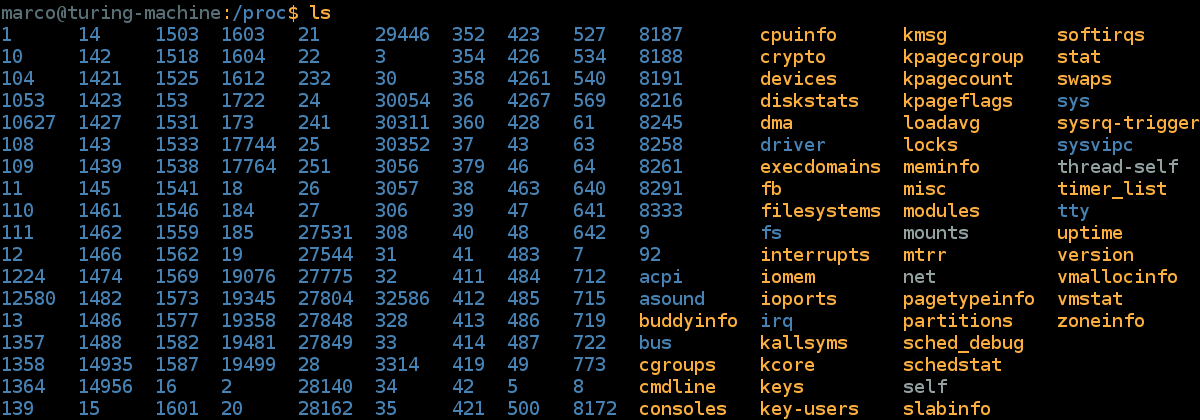
\includegraphics[width=\textwidth]{images/shell_proc.png} 
\caption{The procfs special filesystem}
\label{img:proc}
\end{figure}

If we were to write a user application to display processes; the alternative approach to get this information would be to use a special-purpose syscall, which is what BSD and MacOS do: the syscall will return a kernel structure with all the information that needs to be parsed. The approach used by Linux is more straightforward: the information is (mostly) in human-readable form, so you simply read the files in \verb|/proc| and parse the results as strings. By doing this, you don't need to use any syscall, except, of course, \verb|open()| and \verb|read()| to interact with the filesystem. On Linux, when you use commands like \verb|ps|, \verb|top| or \verb|pgrep|, what they do internally is to query \verb|procfs|. You could always do the same operation manually by doing something like \verb%cat /proc/1337/info_that_you_need | grep specific_info%, but it would be tedious: this is why utilities like \verb|ps| are essentially front-ends for the user.

There are also other specialized filesystems, for example \verb|sysfs|, which contains system information; but what iterests us is \verb|debugfs|, which contains kernel debug information: it's here that we can interact with ftrace. This filesystem is mounted by executing \verb|mount -t debugfs nodev /sys/kernel/debug/|: since there is not an actual device that is being mounted, we use ``\verb|nodev|'' as target device; \verb|/sys/kernel/debug/| is the target mount point. In figure \ref{img:tracing} you can see the trace folder located in this filesystem. To interact with ftrace you simply write in these files with \verb|echo your_value > file|: by doing this you can toggle options and set parameters before/during the trace. 

\begin{figure}[ht]
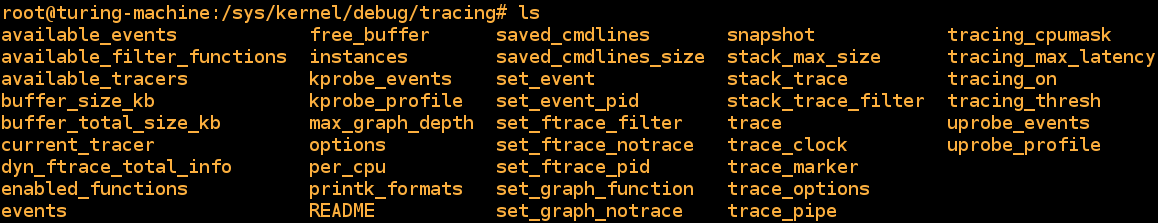
\includegraphics[width=\textwidth]{images/shell_tracing.png} 
\caption{Tracing folder inside the debugfs special filesystem}
\label{img:tracing}
\end{figure}

Some of these files' purpose is not to set options, but rather to list available options. For instance, in figure \ref{img:tracers}, we list the available tracers. These are essentially tracing modes: we activate one by doing \verb|echo function > current_tracer|, which will immediately start the trace with the ``function'' tracer. We can then see the trace output by simply executing \verb|cat trace|. Most of the other files are used for filtering what is being traced, which we will see in detail in the upcoming section.

\begin{figure}[ht]
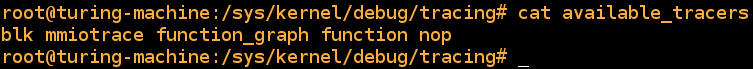
\includegraphics[width=\textwidth]{images/shell_tracers.png} 
\caption{Types of tracers, only a few are available by default on by distribution (Debian)}
\label{img:tracers}
\end{figure}

Let's now see different ways to interact with ftrace:
\begin{codebash}
# Interfacing through an application program
sudo trace-cmd record -p function -P 622
sudo trace-cmd report
# Interfacing through the filesystem
cd /sys/kernel/debug/tracing
echo 622 > set_ftrace_pid
echo function > current_tracer
cat trace
\end{codebash}

This is a good example of the different ways of communication from user to kernel space. In this code, both approaches trace the process with pid 622, and they essentially do it in the same way because \verb|trace-cmd| simply queries \verb|debugfs|, just like \verb|ps| queries \verb|procfs|. We will use the second approach because it shows explicitly how we interface with the kernel, but in practice it's sometimes easier to use tools like \verb|trace-cmd|. Another useful tool is \verb|kernelshark|, which has a GUI to show graphs of the traces done through \verb|trace-cmd|.

\section{Ftrace usage}

\subsection{Function tracing} 
Let's write a simple script that traces any input process.
\begin{codebash}
#!/bin/bash
# traceprocess.sh
echo $$ > /sys/kernel/debug/tracing/set_ftrace_pid
# echo every function to filter
echo __do_page_fault > /sys/kernel/debug/tracing/set_ftrace_filter
echo function > /sys/kernel/debug/tracing/current_tracer
exec $*
\end{codebash}
\verb|$$| is the variable that contains the pid of the script itself, and \verb|$*| are the arguments of the script: in this case, the process to trace. The way it works is very simple:
\begin{enumerate}
    \item Set this pid as the one that will be traced
    \item Set the \verb|__do_page_fault| as the only function to trace
    \item Set the tracer to the function tracer
    \item Execute the input program
    \item The executed program will be a child of the script itself, so its pid will automatically be added to \verb|set_ftrace_pid| and it will be traced
\end{enumerate}
In the kernel, every routine that starts with ``\verb|do_|'' is an interrupt handler: in this case, we traced the interrupt handler for page faults by using a filter. Usually, we would see every kernel function that the input process calls, which is sometimes a big and uninformative output that needs filtering. The trace output can be found in the file \verb|/sys/kernel/debug/tracing/trace|, or can be viewed as it gets written in \verb|/sys/kernel/debug/tracing/trace_pipe|. The following is an output of \verb|./traceprocess.sh ls|, which traces \verb|ls|.
\begin{Verbatim}
# tracer: function
#
# entries-in-buffer/entries-written: 92/92   #P:4
#
#                      _-----=> irqs-off
#                     / _----=> need-resched
#                    | / _---=> hardirq/softirq
#                    || / _--=> preempt-depth
#                    ||| /     delay
#   TASK-PID   CPU#  ||||    TIMESTAMP  FUNCTION
#      | |       |   ||||       |         |
      ls-4973  [000] d... 14386.659663: __do_page_fault <-page_fault
      ls-4973  [000] d... 14386.659718: __do_page_fault <-page_fault
      ls-4973  [000] d... 14386.659743: __do_page_fault <-page_fault
      ls-4973  [000] d... 14386.659784: __do_page_fault <-page_fault
      ls-4973  [000] d... 14386.659800: __do_page_fault <-page_fault
      # ... many more page faults ...
      ls-4973  [000] d... 14386.662473: __do_page_fault <-page_fault
      ls-4973  [000] d... 14386.662871: __do_page_fault <-page_fault
      ls-4973  [000] d... 14386.662881: __do_page_fault <-page_fault
      ls-4973  [000] d... 14386.662900: __do_page_fault <-page_fault
\end{Verbatim}
As expected, we only see page faults (for a total of 92). This information is not that useful by itself, but what is useful, instead, are the timestamps: with these, it's easy to detect latencies in the kernel. By using kernelshark you can plot the trace in order to make latencies obvious; doing this can also be interesting because it lets you see which actions cause most overhead. Another way of doing this just with ftrace is to use the \verb|function_graph| tracer: it's similar to the \verb|function| tracer, but it shows the entry and exit point of each function, creating a function call graph. Instead of timestamps it shows the duration of each function execution. The symbols \verb|+|, \verb|!| \verb|#| are used whenever there is an execution time greater than 10, 100 and 1000 microseconds. As we know, scheduling and thread migration cause a lot of overhead, so we can try to use \verb|function_graph| to see it.
\begin{Verbatim}
 2)               |            schedule() {
 2)   0.033 us    |              rcu_note_context_switch();
 2)   0.028 us    |              _raw_spin_lock();
 2)               |              deactivate_task() {
 2)   0.032 us    |                update_rq_clock.part.84();
 2)               |                dequeue_task_fair() {
 2)               |                  dequeue_entity() {
 2)               |                    update_curr() {
 2)   0.030 us    |                      update_min_vruntime();
 2)   0.060 us    |                      cpuacct_charge();
 2)   0.654 us    |                    }
 2)   0.029 us    |                    clear_buddies();
 2)   0.033 us    |                    account_entity_dequeue();
 2)   0.041 us    |                    update_cfs_shares();
 2)   0.027 us    |                    update_min_vruntime();
 2)   2.188 us    |                  }
 2)   0.030 us    |                  hrtick_update();
 2)   2.767 us    |                }
 2)   3.362 us    |              }
 2)               |              pick_next_task_fair() {
 2)   0.028 us    |                __msecs_to_jiffies();
 2)   0.353 us    |              }
 2)               |              pick_next_task_idle() {
 2)               |                put_prev_task_fair() {
 2)               |                  put_prev_entity() {
 2)   0.029 us    |                    check_cfs_rq_runtime();
 2)   0.323 us    |                  }
 2)   0.608 us    |                }
 2)   0.036 us    |                update_idle_core();
 2)   1.208 us    |              }
 2)   0.033 us    |      finish_task_switch();
 2) ! 114.732 us  |    } /* schedule */
 2) ! 115.042 us  |  } /* schedule_preempt_disabled */
\end{Verbatim}
This is small piece of a trace of every function call on my system, without function or process filters. Function duration is located at every leaf function and function exit point (\verb|}|): as you can see \verb|schedule()| takes longer to execute than the other functions; there is also a \verb|!| because it's more that 100 microseconds. As we said earlier, the buffer can be filled and some entries will be lost: this is very common if you trace everything without filtering, which is what we did here. 

The ftrace documentation says ``The function name is always displayed after the closing bracket for a function if the start of that function is not in the trace buffer''. In our case, this means that the exit point ``\verb|} /* schedule */|'' is not referring to the initial \verb|schedule()| entry point! Even though we can see the overhead of the function, the actual entry point is not there because it couldn't get written in the trace. To mitigate this we can trace on a single CPU, instead of all 4. This approach has three advantages: 
\begin{itemize}
    \item The output won't have function calls interleaved between the CPUs, which breaks the flow of function calls
    \item Since fewer entries are traced, the buffer won't be filled and many won't be lost
    \item There is a performance gain: tracing every single function call generates significant overhead
\end{itemize}
In general, it's better to narrow the filters as much as possible. For example, it would be good to trace only the function that we're interested in, and on one CPU only: in the next chapter, we will always trace this way in order to reduce noise.

Let's try to trace only the \verb|schedule()| function, on all CPUS, just to see how much time it can take (on my machine, that is). We do this by executing: 
\begin{codebash}
cd /sys/kernel/debug/tracing/
echo schedule > set_graph_function
cat trace | grep -F "/* schedule */"
\end{codebash}
The output is:
\begin{Verbatim}
+ means that the function exceeded 10 usecs.
! means that the function exceeded 100 usecs.
# means that the function exceeded 1000 usecs.
* means that the function exceeded 10 msecs.
@ means that the function exceeded 100 msecs.
$ means that the function exceeded 1 sec.

 2) + 58.121 us   |  } /* schedule */
 1) + 68.348 us   |  } /* schedule */
 2) @ 991933.0 us |      } /* schedule */
 1) @ 992178.9 us |      } /* schedule */
 1) * 31760.76 us |      } /* schedule */
 3) ! 139.005 us  |  } /* schedule */
 3) $ 1147687 us  |      } /* schedule */
 2) + 49.196 us   |  } /* schedule */
 3) # 1243.739 us |  } /* schedule */
 2) * 97870.13 us |  } /* schedule */
 0) + 39.666 us   |  } /* schedule */
 3) + 63.518 us   |  } /* schedule */
 0) # 1193.975 us |  } /* schedule */
 0) ! 345.386 us  |  } /* schedule */
 3) + 74.291 us   |  } /* schedule */
 0) # 1381.706 us |  } /* schedule */
 0) ! 113.232 us  |  } /* schedule */
 0) ! 106.633 us  |  } /* schedule */
 2) # 1652.529 us |  } /* schedule */
 1) $ 1023917 us  |      } /* schedule */
 3) @ 935896.8 us |      } /* schedule */
 2) $ 1123576 us  |      } /* schedule */
 1) * 67530.47 us |      } /* schedule */
 0) + 88.367 us   |  } /* schedule */
 1) # 1585.574 us |  } /* schedule */
 2) @ 231657.1 us |      } /* schedule */
 2) ! 389.683 us  |  } /* schedule */
 0) + 70.527 us   |  } /* schedule */
 1) # 1461.529 us |  } /* schedule */
 3) ! 120.510 us  |  } /* schedule */
 0) + 90.422 us   |  } /* schedule */
 2) # 1433.207 us |  } /* schedule */
 2) @ 307235.2 us |      } /* schedule */
 3) $ 1063775 us  |  } /* schedule */
\end{Verbatim}
%Cerca di capire perchè succede e spiegalo 
%tracing_cpumask?
The output is not the average time, but rather an unordered mix with a prevalence of the longest times recorded. The reason is that we looked for commented exit points, so these are actually only the exit points that don't have an entry point in the trace (as stated by the documentation). There are some cases where it took more than 1 second (``\verb|$|'') to execute: these are extreme cases where the schedule got interruped and some other kernel task was done in the meantime, so it didn't actually take a whole second \textbf{just} to schedule. If we look for every exit point---not just the orphaned ones---we can see that on average the \verb|schedule()| routine will take less time, but still more than the other functions.

There is also another problem with this trace. Steven Rostedt, the creator of ftrace, said in one of its articles that ``Only the leaf functions, the ones that do not call other functions, have an accurate duration, since the duration of parent functions also includes the overhead of the \verb|function_graph| tracer calling the child functions''.\cite{secrets} This means that taking the difference between the timestamp of the entry and exit point is not enough, since the overhead of ftrace is not taken into account. The same article says ``By using the \verb|set_ftrace_filter| file, you can force any function into becoming a leaf function in the \verb|function_graph| tracer, and this will allow you to see an accurate duration of that function''. If we do that we find out, more accurately, that most of the time it will take between $20 \mu s$ and $400\mu s$ to execute \verb|schedule()|.

\subsection{Event tracing}
Function tracing is very useful and will come in handy to understand the code, but now we will focus on events. You may have noticed in figure \ref{img:tracing} that there is a directory called ``events''. It contains a folder for each \textit{event subsystem}, and the one we're interested in is \verb|sched|, for the scheduling subsystem. Figure \ref{img:sched} shows its contents: there is a folder for each event, containing information about it and a switch to enable/disable it. This is essentially a list of the events that we're going to document, even though some of their names are almost self explainatory.

\begin{figure}[ht]
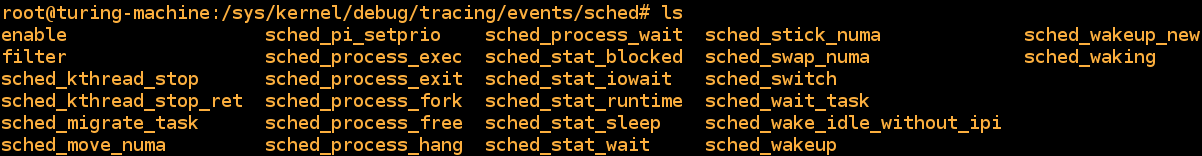
\includegraphics[width=\textwidth]{images/shell_sched.png}
\caption{Every event associated with scheduling}
\label{img:sched}
\end{figure}

\begin{figure}[ht]
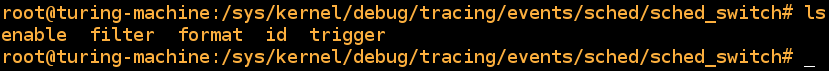
\includegraphics[width=\textwidth]{images/shell_sched_event.png} 
\caption{Control files for the sched\_switch event}
\label{img:sched_event}
\end{figure}

So what are events, exactly? As anticipated, event tracing is much more static compared to function tracing. What this means is that event \textit{tracepoints} are directly embedded in the code and are called just like functions, so they cannot be toggled at runtime and you need to recompile the whole kernel to change/disable them. From this perspective, events are really similar to regular prints, but in practice events are much more efficient than \verb|printk()|. 

Steven Rostedt explains pretty well why that is the case: 
``\verb|printk()| is the king of all debuggers, but it has a problem. If you are debugging a high volume area such as the timer interrupt, the scheduler, or the network, \verb|printk()| can lead to bogging down the system or can even create a live lock. It is also quite common to see a bug ``disappear'' when adding a few \verb|printk()|s. This is due to the sheer overhead that \verb|printk()| introduces. Ftrace introduces a new form of \verb|printk()| called \verb|trace_printk()|. It can be used just like \verb|printk()|, and can also be used in any context (interrupt code, NMI code, and scheduler code). What is nice about \verb|trace_printk()| is that it does not output to the console. Instead it writes to the Ftrace ring buffer and can be read via the trace file. Writing into the ring buffer with \verb|trace_printk()| only takes around a tenth of a microsecond or so. But using \verb|printk()|, especially when writing to the serial console, may take several milliseconds per write.''\cite{trace_debugging} \verb|trace_printk()| simply writes a message in the trace buffer, which is exactly what happens with events, just with a pre-defined format and many printed fields. Because of this, what is said in the quote also applies to events. In figure \ref{img:sched_event_format} you can see how similar to a print an event actually is. Each event has this format file which states fields and print formatting, with the same syntax of \verb|printk()|. In the upcoming section, we will see how to declare these properties for an event from the kernel.

\begin{figure}[ht]
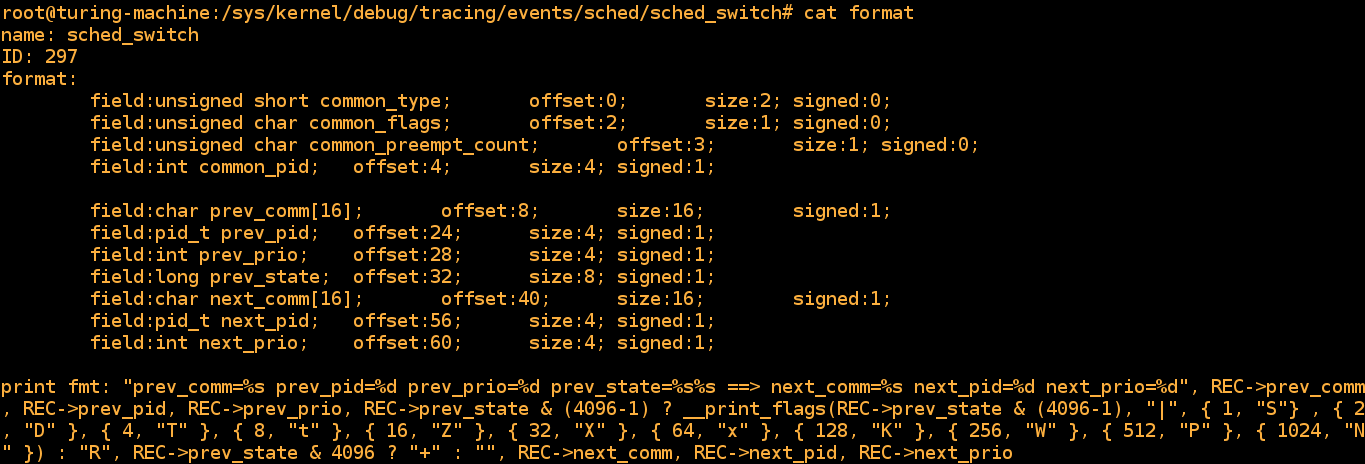
\includegraphics[width=\textwidth]{images/shell_sched_event_format.png} 
\caption{Fields and print format of the sched\_switch event}
\label{img:sched_event_format}
\end{figure}

Let's now see how event tracing is enabled and how to filter events. Events are not related with any tracer because tracers are used for dynamic tracing only. If we want to see just the events, then we must use the \verb|nop| tracer (which doesn't trace anything), but we could also trace events while tracing functions by enabling any other tracer. 

\begin{codebash}
# enable scheduling events
echo nop > /sys/kernel/debug/tracing/current_tracer
echo 1 > /sys/kernel/debug/tracing/events/sched/enable
# enable just the sched_switch event
echo nop > /sys/kernel/debug/tracing/current_tracer
echo 1 > /sys/kernel/debug/tracing/events/sched/sched_switch/enable
\end{codebash}

The ``enable'' file is located in every folder of the event directory tree. As you can see, the directory hierarchy is used to toggle single events, entire event subsystems, or all the existing events. Be aware that this filter doesn't stop the events from being written in the trace buffer, we are just ignoring them. ``You have to recompile the whole kernel to disable specific events'' can be paraphrased as ``You have to recompile the whole kernel to prevent ftrace from writing specific events in its buffer, even when they are disabled from \verb|debugfs|''.

The following is a small piece of a trace of every scheduling event:

\begin{Verbatim}[xleftmargin=-2cm,fontsize=\footnotesize]
# tracer: nop
#
# entries-in-buffer/entries-written: 116546/459475   #P:4
#
#                      _-----=> irqs-off
#                     / _----=> need-resched
#                    | / _---=> hardirq/softirq
#                    || / _--=> preempt-depth
#                    ||| /     delay
#   TASK-PID   CPU#  ||||    TIMESTAMP  FUNCTION
#      | |       |   ||||       |         |
  <idle>-0     [000] d...   611.283814: sched_switch: prev_comm=swapper/0 prev_pid=0 prev_prio=120 prev_state=R ==> next_comm=Xorg next_pid=1450 next_prio=120
    Xorg-1450  [000] d...   611.283921: sched_stat_runtime: comm=Xorg pid=1450 runtime=117083 [ns] vruntime=17539094302 [ns]
    Xorg-1450  [000] d...   611.283924: sched_switch: prev_comm=Xorg prev_pid=1450 prev_prio=120 prev_state=S ==> next_comm=swapper/0 next_pid=0 next_prio=120
  <idle>-0     [000] d...   611.283957: sched_switch: prev_comm=swapper/0 prev_pid=0 prev_prio=120 prev_state=R ==> next_comm=Xorg next_pid=1450 next_prio=120
    # ... many more entries ...
\end{Verbatim}
In this trace, the swapper process (pid 0) was switched out to schedule Xorg, which is the display server (essentially, the GUI) of the system, and then back again to the swapper; all in a matter of $143 \mu s$. \verb|sched_switch| and \verb|sched_stat_runtime| are the most common scheduling events. The first reports when a process switch happens, by printing information about the old and new process, and the second prints core scheduling information of the running process, such as pid, actual runtime and virtual runtime. The tracepoints for these events look like this in the code:
\begin{code}
trace_sched_switch(preempt, prev, next);
trace_sched_stat_runtime(curtask, delta_exec, curr->vruntime);
\end{code}
As we said earlier, every information printed out in the trace is found through the parameters.

\section{Creating new events}

Tracepoints are created from within the kernel. At this level, events are seen as structures which carry the information needed for the event. A tracepoint must create this structure, fill it with data and write it in the ftrace ring buffer. So, this buffer is basically an array of binary data, which will be periodically consumed, decoded and printed as a string in the trace output.

Besides the core infrastructure of ftrace, its developers have also made iterfaces to make it easy for kernel developers to create tracepoints. Today, this process is almost completely automated thanks to the \verb|TRACE_EVENT()| macro and other sub-macros called by it. By using \verb|TRACE_EVENT()| it's possible to quickly create tracepoints in the core kernel code, or even in a kernel module, without much boilerplate code. Every existing tracepoint for scheduling events is created by using this macro: these tracepoints are declared in a separate, dedicated, header file, which is then included in the main code. The default path for these headers is \verb|include/trace/events|, so the declarations for the scheduling events are in \verb|include/trace/events/sched.h|. Let's see what's in this header.

\begin{code}
#undef TRACE_SYSTEM
#define TRACE_SYSTEM sched
#if !defined(_TRACE_SCHED_H) || defined(TRACE_HEADER_MULTI_READ) // Special guard
#define _TRACE_SCHED_H
// ... some other includes ...
#include <linux/tracepoint.h> //TRACE_EVENT() defined in here, then redefined at the end of this trace header
/*
 * Tracepoint for a task being migrated:
 */
TRACE_EVENT(sched_migrate_task,
	TP_PROTO(struct task_struct *p, int dest_cpu),
	TP_ARGS(p, dest_cpu),
	TP_STRUCT__entry(
		__array(char, comm,	TASK_COMM_LEN)
		__field(pid_t, pid)
		__field(int, prio)
		__field(int, orig_cpu)
		__field(int, dest_cpu)
	),
	TP_fast_assign(
		memcpy(__entry->comm, p->comm, TASK_COMM_LEN);
		__entry->pid = p->pid;
		__entry->prio = p->prio; /* XXX SCHED_DEADLINE */
		__entry->orig_cpu = task_cpu(p);
		__entry->dest_cpu = dest_cpu;
	),
	TP_printk("comm=%s pid=%d prio=%d orig_cpu=%d dest_cpu=%d",
		  __entry->comm, __entry->pid, __entry->prio,
		  __entry->orig_cpu, __entry->dest_cpu)
);
// ... many more event declarations ...
#endif /* _TRACE_SCHED_H */
/* This part must be outside protection */
#include <trace/define_trace.h>
\end{code}

The whole file is basically a list of declarations like this one. This is the declaration of \verb|sched_migrate_task|, which was shown in section \ref{sec:how_does_it_work}. These weird includes at the end of the file and the special guard have something to do with how \verb|TRACE_EVENT()| works internally; we will give a brief overview of that at the end of the section. The macro itself has 6 parameters, with 5 different sub-macros:
\begin{itemize}
    \item The first is the tracepoint name, the final name will have the format \verb|trace_NAME|.
    \item \verb|TP_PROTO| and \verb|TP_ARGS| simply define the arguments of the tracepoint
    \item \verb|TP_STRUCT__entry| defines the struct of the event, with every attribute type and name. There are 2 different sub-sub-macros to define fields and arrays.
    \item \verb|TP_fast_assign| defines how to fill the event struct, usually with the event parameters. This is not trivial because they can be filled by using other functions, macros or by \verb|memcpy()|, \verb|memmove()| etc...
    \item \verb|TP_printk| has the same syntax of \verb|printk()| and defines how to print the struct in human-readable form in the trace output. In the examples at the beginning of this section, you can see that \verb|sched_migrate_task| is printed just like that.
\end{itemize}

The format defined with \verb|TP_printk| can be seen from user space in the ``format'' subfolder in the event directory, as seen in figure \ref{img:sched_event_format}. \verb|TRACE_SYSTEM| is the trace system of the events, this will spawn the folder in the events directory and use it for these events: in figure \ref{img:systems} you can see the ``sched'' folder declared in the header, and its content in figure \ref{img:sched}, where there is also \verb|sched_migrate_task|. 
\begin{figure}[ht]
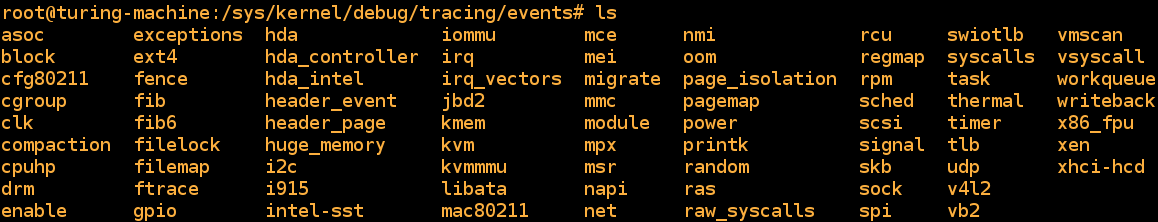
\includegraphics[width=\textwidth]{images/shell_trace_systems.png} 
\caption{All of the systems in which events are subdivided}
\label{img:systems}
\end{figure}

\subsection{Kernel module to test tracepoints}
\label{sec:module}
Let's create our own kernel module, which will do something that we can trace from outside the kernel.
\begin{code}
#include <linux/module.h>
#include <linux/kthread.h>
#define CREATE_TRACE_POINTS
#include "my_module_trace.h"

static int do_stuff(void *arg){
	struct task_struct * p = current;
	u64 count = 0;
	printk(KERN_INFO "Current process is %s with pid %d\n", current->comm, current->pid);
	while (!kthread_should_stop()){
		set_current_state(TASK_INTERRUPTIBLE);
		schedule_timeout(HZ);
		printk("hi! %llu\n", count);
		count++;
		trace_my_event(p, jiffies); //Tracepoint
		p = next_task(p);
	}
	return 0;
}

static struct task_struct *my_tsk;
static int __init init_func(void){
	u32 i = 0, j = 0;
	struct task_struct *p, *t;
	printk(KERN_INFO "Hello world\n");
	for_each_process(p){
		i++;
		for_each_thread(p, t){
			j++;
		}
	}
	printk(KERN_INFO "There are %d processes\n", i);
	printk(KERN_INFO "There are %d threads\n", j);
	//printk(KERN_INFO "Average threads per process: %s\n", division_hack(j, i));
	printk(KERN_INFO "Current process is %s with pid %d\n", current->comm, current->pid);
	
	my_tsk = kthread_run(do_stuff, NULL, "my-kthread");
	if (IS_ERR(my_tsk))
		return -1;
	return 0;
}

static void __exit exit_func(void){
	kthread_stop(my_tsk);
	printk(KERN_INFO "Goodbye world\n");
}

module_init(init_func);
module_exit(exit_func);
MODULE_LICENSE("GPL");
\end{code}
This is the trace header \verb|my_module_trace.h| included in the module:
\begin{code}
#undef TRACE_SYSTEM
#define TRACE_SYSTEM my_system
#if !defined(_MY_MODULE_TRACE_H) || defined(TRACE_HEADER_MULTI_READ) // Special guard
#define _MY_MODULE_TRACE_H
#include <linux/tracepoint.h> // TRACE_EVENT() is defined here
TRACE_EVENT(my_event,
	TP_PROTO(struct task_struct * t, unsigned long ticks),
	TP_ARGS(t, ticks),
	TP_STRUCT__entry(
		__array(char, name, TASK_COMM_LEN)
		__field(pid_t, pid)
		__field(u64, vruntime)
		__field(unsigned long, ticks)
	),
	TP_fast_assign(
		memcpy(__entry->name, t->comm, TASK_COMM_LEN);
		__entry->pid	= t->pid;
		__entry->vruntime = t->se.vruntime;
		__entry->ticks = ticks;
	),
	TP_printk("name=%s pid=%d vruntime=%lli ticks=%li", __entry->name,
	__entry->pid, __entry->vruntime, __entry->ticks)
);
#endif /* _MY_MODULE_TRACE_H */
/* This part must be outside protection */
#undef TRACE_INCLUDE_PATH
#define TRACE_INCLUDE_PATH .
#define TRACE_INCLUDE_FILE my_module_trace
#include <trace/define_trace.h>
\end{code}
We can compile by linking the headers of the currently running kernel on the system: these can be found within user space in \verb|/lib/modules/your-kernel-version/build/include|. We then insert the module with \verb|sudo insmod my_module.ko|, then we print the kernel log with \verb|sudo dmesg|: here we can see our \verb|printk()| output.
\begin{Verbatim}
[  410.661000] Hello world
[  410.661062] There are 160 processes
[  410.661065] There are 437 threads
[  410.661067] Current process is insmod with pid 5637
[  410.661111] Current process is my-kthread with pid 5638
[  411.683260] hi! 0
[  412.707226] hi! 1
[  413.731156] hi! 2
[  414.755236] hi! 3
# ...
\end{Verbatim}
We essentially used kernel APIs defined in the included headers. \verb|for_each_process()|, \verb|for_each_thread()| and \verb|current| are all macros which are also used in the scheduler code. \verb|init_func()| is the initialization function executed upon module insertion, so when we first print the currently executing process we read \verb|insmod|. We then spawn a kernel thread which goes in a sleep state and wakes up after \verb|HZ| ticks (one second); it then prints hi and throws an event before going into sleep again. We remove the module with \verb|sudo rmmod my_module|, so \verb|exit_func()| is executed, the kthread is terminated and the module removed.

We said earlier that bugs in the kernel can lock the system or in the worst case corrupt your data: this is why kernel modules are usually tested in a virtual machine, and the same goes for core kernel code. For example, in our module lines 11 and 12 are important: if we comment them out, the system completely freezes after a couple of seconds upon module insertion, and then crashes. What happens is that the thread hogs the CPU, starving all other processes: it can do this without being preempted because it's a kernel thread. While kernel threads are scheduled like normal tasks, it's also true that if they don't yield the CPU voluntarily, then they can continue to execute almost indefinitely. This is due to their priority being higher than most processes running on the system.
While hogging the CPU, messages like this can be read in the kernel log:
\begin{Verbatim}
[ 2795.881548] NMI watchdog: BUG: soft lockup - CPU#3 stuck for 22s! [my-kthread:2921]    
\end{Verbatim}
Because of \verb|TRACE_EVENT()|, we now have a folder for our trace system. We can trace our event by simply doing \verb|echo 1 > trace/events/my_system/enable| in \verb|debugfs|. The following is the trace output:
\begin{Verbatim}[xleftmargin=-2cm,fontsize=\footnotesize]
# tracer: nop
#
# entries-in-buffer/entries-written: 191/191   #P:4
#
#                        _-----=> irqs-off
#                       / _----=> need-resched
#                      | / _---=> hardirq/softirq
#                      || / _--=> preempt-depth
#                      ||| /     delay
#   TASK - PID   CPU#  ||||    TIMESTAMP  FUNCTION
#      |   |       |   ||||       |         |
my-kthread-5638  [001] ....   411.683267: my_event: name=my-kthread pid=5638 vruntime=52137176502 ticks=4294995168
my-kthread-5638  [001] ....   412.707241: my_event: name=swapper/0 pid=0 vruntime=0 ticks=4294995424
my-kthread-5638  [001] ....   413.731163: my_event: name=systemd pid=1 vruntime=50883640967 ticks=4294995680
my-kthread-5638  [001] ....   414.755245: my_event: name=kthreadd pid=2 vruntime=52053628354 ticks=4294995936
my-kthread-5638  [002] ....   415.779197: my_event: name=ksoftirqd/0 pid=3 vruntime=53378623957 ticks=4294996192
my-kthread-5638  [002] ....   416.803364: my_event: name=kworker/0:0H pid=5 vruntime=722463814 ticks=4294996448
my-kthread-5638  [003] ....   417.831200: my_event: name=kworker/u8:0 pid=6 vruntime=44397385655 ticks=4294996705
my-kthread-5638  [003] ....   418.851389: my_event: name=rcu_sched pid=7 vruntime=52699580435 ticks=4294996960
my-kthread-5638  [003] ....   419.875192: my_event: name=rcu_bh pid=8 vruntime=62278851 ticks=4294997216
my-kthread-5638  [001] ....   420.903141: my_event: name=migration/0 pid=9 vruntime=0 ticks=4294997473
my-kthread-5638  [001] ....   421.923231: my_event: name=lru-add-drain pid=10 vruntime=67280643 ticks=4294997728
my-kthread-5638  [001] ....   422.947183: my_event: name=watchdog/0 pid=11 vruntime=-5995840 ticks=4294997984
my-kthread-5638  [001] ....   423.971192: my_event: name=cpuhp/0 pid=12 vruntime=1485464677 ticks=4294998240
my-kthread-5638  [001] ....   424.995245: my_event: name=cpuhp/1 pid=13 vruntime=1137933842 ticks=4294998496
my-kthread-5638  [002] ....   426.019248: my_event: name=watchdog/1 pid=14 vruntime=-2923868 ticks=4294998752
my-kthread-5638  [002] ....   427.043155: my_event: name=migration/1 pid=15 vruntime=0 ticks=4294999008
my-kthread-5638  [000] ....   428.067198: my_event: name=ksoftirqd/1 pid=16 vruntime=53693736956 
# ... more entries ...
my-kthread-5638  [003] ....   552.996462: my_event: name=su pid=1598 vruntime=5158411963 ticks=4295030496
my-kthread-5638  [003] ....   554.020544: my_event: name=bash pid=1619 vruntime=66899459134 ticks=4295030752
my-kthread-5638  [003] ....   555.044561: my_event: name=firefox-esr pid=1684 vruntime=68424773099 ticks=4295031008
my-kthread-5638  [003] ....   556.068429: my_event: name=Web Content pid=1741 vruntime=68730788669 ticks=4295031264
my-kthread-5638  [003] ....   557.092489: my_event: name=nemo pid=1837 vruntime=66762475178 ticks=4295031520
my-kthread-5638  [003] ....   558.116460: my_event: name=gvfsd-metadata pid=1852 vruntime=7178686451 ticks=4295031776
my-kthread-5638  [003] ....   559.140545: my_event: name=dconf-service pid=1860 vruntime=7166782392 ticks=4295032032
my-kthread-5638  [003] ....   560.164474: my_event: name=Telegram pid=1912 vruntime=69024257689 ticks=4295032288
my-kthread-5638  [003] ....   561.188485: my_event: name=avahi-autoipd pid=2017 vruntime=56548711450 ticks=4295032544
my-kthread-5638  [003] ....   562.212523: my_event: name=avahi-autoipd pid=2018 vruntime=11116028299 ticks=4295032800
my-kthread-5638  [003] ....   563.236617: my_event: name=dhclient pid=2115 vruntime=66126515993 ticks=4295033056
\end{Verbatim}
It iterates through the process list, each second printing information about a process. It first traces the kernel threads (low pid), and eventually finds the user processes. 
\subsection{Overview of \texttt{TRACE\_EVENT()} infrastructure}
The macro works by expanding many other sub-macros. What it needs to do is to generate the structs and then generate the code of the tracepoint function, which basically writes the event in the trace ring buffer. To accomplish that, the marco uses a C pre-processor trick that lets you change its behavior while using the same input data. Here is a perfect example from yet another Steven Rostedt article:\cite{trace_event}
\begin{code}
#define DOGS { C(JACK_RUSSELL), C(BULL_TERRIER), C(ITALIAN_GREYHOUND) }
#undef C
#define C(a) ENUM_##a
enum dog_enums DOGS;
#undef C
#define C(a) #a
char *dog_strings[] = DOGS;
char *dog_to_string(enum dog_enums dog)
{
       return dog_strings[dog];
}
\end{code}
By redefining the sub-macro \verb|C(a)| throughout the program, we change the behavior of \verb|DOGS|: this way, we generate different code with the same data. \verb|TRACE_EVENT()| does the same with its parameters, but performs this trick in a really weird way. Imagine that we had two different headers: \verb|generate_code.h| and \verb|change_behavior.h|. \\\verb|generate_code.h|:
\begin{enumerate}
    \item Uses the macro, expanding it and generating code with a given input data
    \item Does \verb|#include change_behavior.h|
\end{enumerate}
\verb|change_behavior.h|:
\begin{enumerate}
    \item Redefines the sub-macros, changing the original macro's behavior
    \item Does \verb|#include generate_code.h|, reincluding the header that just included it, which will generate new code
    \item Repeats the process many times
\end{enumerate}
This is exactly what we did with \verb|DOGS|, it's just not as easy to see what happens. With this technique it's easier to change the macro usage because we have two separate files, but the code is way harder to read. Let's use our module to illustrate the mechanism in actual kernel code.\\\verb|my_module|:
\begin{code}
#define CREATE_TRACE_POINTS
#include "my_module_trace.h"
\end{code}
\verb|CREATE_TRACE_POINTS| is defined only if the kernel was compiled with the trace option activated.\\\verb|my_module_trace.h|:
\begin{code}
#if !defined(_MY_MODULE_TRACE_H) || defined(TRACE_HEADER_MULTI_READ) // Special guard
#define _MY_MODULE_TRACE_H
#include <linux/tracepoint.h> //TRACE_EVENT() is defined here
TRACE_EVENT(my_event, ..., ..., ..., ..., ...)
// ... All other event declarations ...
#endif /* _MY_MODULE_TRACE_H */
/* This part must be outside protection */
#undef TRACE_INCLUDE_PATH
#define TRACE_INCLUDE_PATH .
#define TRACE_INCLUDE_FILE my_module_trace
#include <trace/define_trace.h>
\end{code}
This is the file that uses \verb|TRACE_EVENT()| and the special guard is what makes us able to reinclude it multiple times. Usually, a guard is used to avoid mutiple inclusions. This is because if a function declaration is included twice, then we can't compile since there are two functions with the same name. Since there are no functions in trace headers, but just macros, then it's perfectly safe (and in this case needed) to do multiple inclusions. For reference, this would be the common use of a guard:
\begin{code}
#ifndef _MY_MODULE_TRACE_H
#define _MY_MODULE_TRACE_H
// ... Code ...
#endif _MY_MODULE_TRACE_H
\end{code}
At the end of the file, we define two more macros. \verb|TRACE_INCLUDE_FILE| is the name of this file, which is needed later for the reinclusion. \verb|TRACE_INCLUDE_PATH| changes the path of the trace headers, in this case it's \verb|.| to indicate the current folder. This is needed for modules because they never use the default path used for core kernel code (\verb|include/trace/events/|). This information is also needed for the reinclusion, which is performed in the header \verb|define_trace.h| included at the end: this header corresponds to the ``\verb|change_behavior.h|'' mentioned earlier.\\\verb|define_trace.h|:
\begin{code}
#ifdef CREATE_TRACE_POINTS // Defined to activate the tracepoints, used here as a guard
/* Prevent recursion */
#undef CREATE_TRACE_POINTS
// ... Redefine the sub-macros to change the behavior ...

#ifndef TRACE_INCLUDE_FILE
# define TRACE_INCLUDE_FILE TRACE_SYSTEM
# define UNDEF_TRACE_INCLUDE_FILE
#endif

#ifndef TRACE_INCLUDE_PATH
# define __TRACE_INCLUDE(system) <trace/events/system.h> //Used to reread system.h (e.g.: sched.h) trace header
# define UNDEF_TRACE_INCLUDE_PATH
#else
# define __TRACE_INCLUDE(system) __stringify(TRACE_INCLUDE_PATH/system.h)
#endif

# define TRACE_INCLUDE(system) __TRACE_INCLUDE(system)

/* Let the trace headers be reread */
#define TRACE_HEADER_MULTI_READ 
// Reinclusion: includes the file that just included it
// e.g.: if the subsystem was sched, this just included <trace/events/sched.h>, in our example it's <./my_module_trace.h>
#include TRACE_INCLUDE(TRACE_INCLUDE_FILE) 
#ifdef TRACEPOINTS_ENABLED
#include <trace/trace_events.h>
#endif
// ... Undefine every single macro and sub-macro ...

/* We may be processing more files */
#define CREATE_TRACE_POINTS
#endif /* CREATE_TRACE_POINTS */
\end{code}
Before the reinclusion, it's important to undefine \verb|CREATE_TRACE_POINTS|, causing the guard to activate. This is because the reincluded file (\verb|my_module_trace.h|) could include again this file (\verb|define_trace.h|) at the end, causing an infinite loop in compilation. The next sequence generates the path of the file that included this file, taking the information from \verb|TRACE_SYSTEM|, \verb|TRACE_INCLUDE_FILE| and \verb|TRACE_INCLUDE_PATH|. Finally, the file in the generated path is reincluded, causing \verb|TRACE_EVENT()| to generate different code. At the end, \verb|trace_events.h| is included: this header simply does this process again, many times. Its code has this general structure:
\begin{code}
// Stage 1: change behavior
#include TRACE_INCLUDE(TRACE_INCLUDE_FILE) // Generate
// Stage 2: change behavior
#include TRACE_INCLUDE(TRACE_INCLUDE_FILE) // Generate
// Stage 3: change behavior
#include TRACE_INCLUDE(TRACE_INCLUDE_FILE) // Generate
// ...
\end{code}
Each stage simply redefines the sub-macros to generate code for a specific purpose. This is not exactly how the stages are structured, but just as an example, the stages could generate code like this:
\begin{itemize}
    \item Stage 1: Generates the event struct with the proper fields
    \item Stage 2: Generates a struct with the offsets of each field in the event struct
    \item Stage 3: Creates the folder in the event directory of \verb|debugfs|
    \item Stage 4: Generates a function that prints the raw event in the trace output format
    \item Stage 5: Generates a function to write the struct in the ring buffer
\end{itemize}
That's it! The code in this file is not hard to understand, it's just hard to read. There is also a big amount of code, and that's also why we are not going to go through it. For our purposes, that is not really interesting, but what really is interesting is how \verb|TRACE_EVENT()| it's structured (and how hacky it is). For the curious, the path is \verb|include/trace/events/trace_events.h|.

